% 图 77.1 —— 由 `checks/emit_hand.py` 自动拼出（probe 精测 + prims2 图元分解）
%%
% ⚠ 这是**稿子不是成品**：跑 `checks/checkhand.py 77.1` 看指标 + 看叠合图。
%%
%% ⚠ 待核：
%   · 本图 probe 报出阴影族 3 个 —— **本脚本不生成阴影**（要照原书手写）；prims2 的 strokes 里可能含阴影线，核对时留意别画重
%   · 可疑字形 1 项（空心圈 ⊙ 常被认成字母 o）—— 见文件末
%%
\documentclass[12pt]{standalone}
\usepackage{fontspec}
\setsansfont{Arial}
\newfontfamily\mfallback{DejaVu Sans}
\usepackage{tikz}
\usetikzlibrary{arrows.meta}
\begin{document}
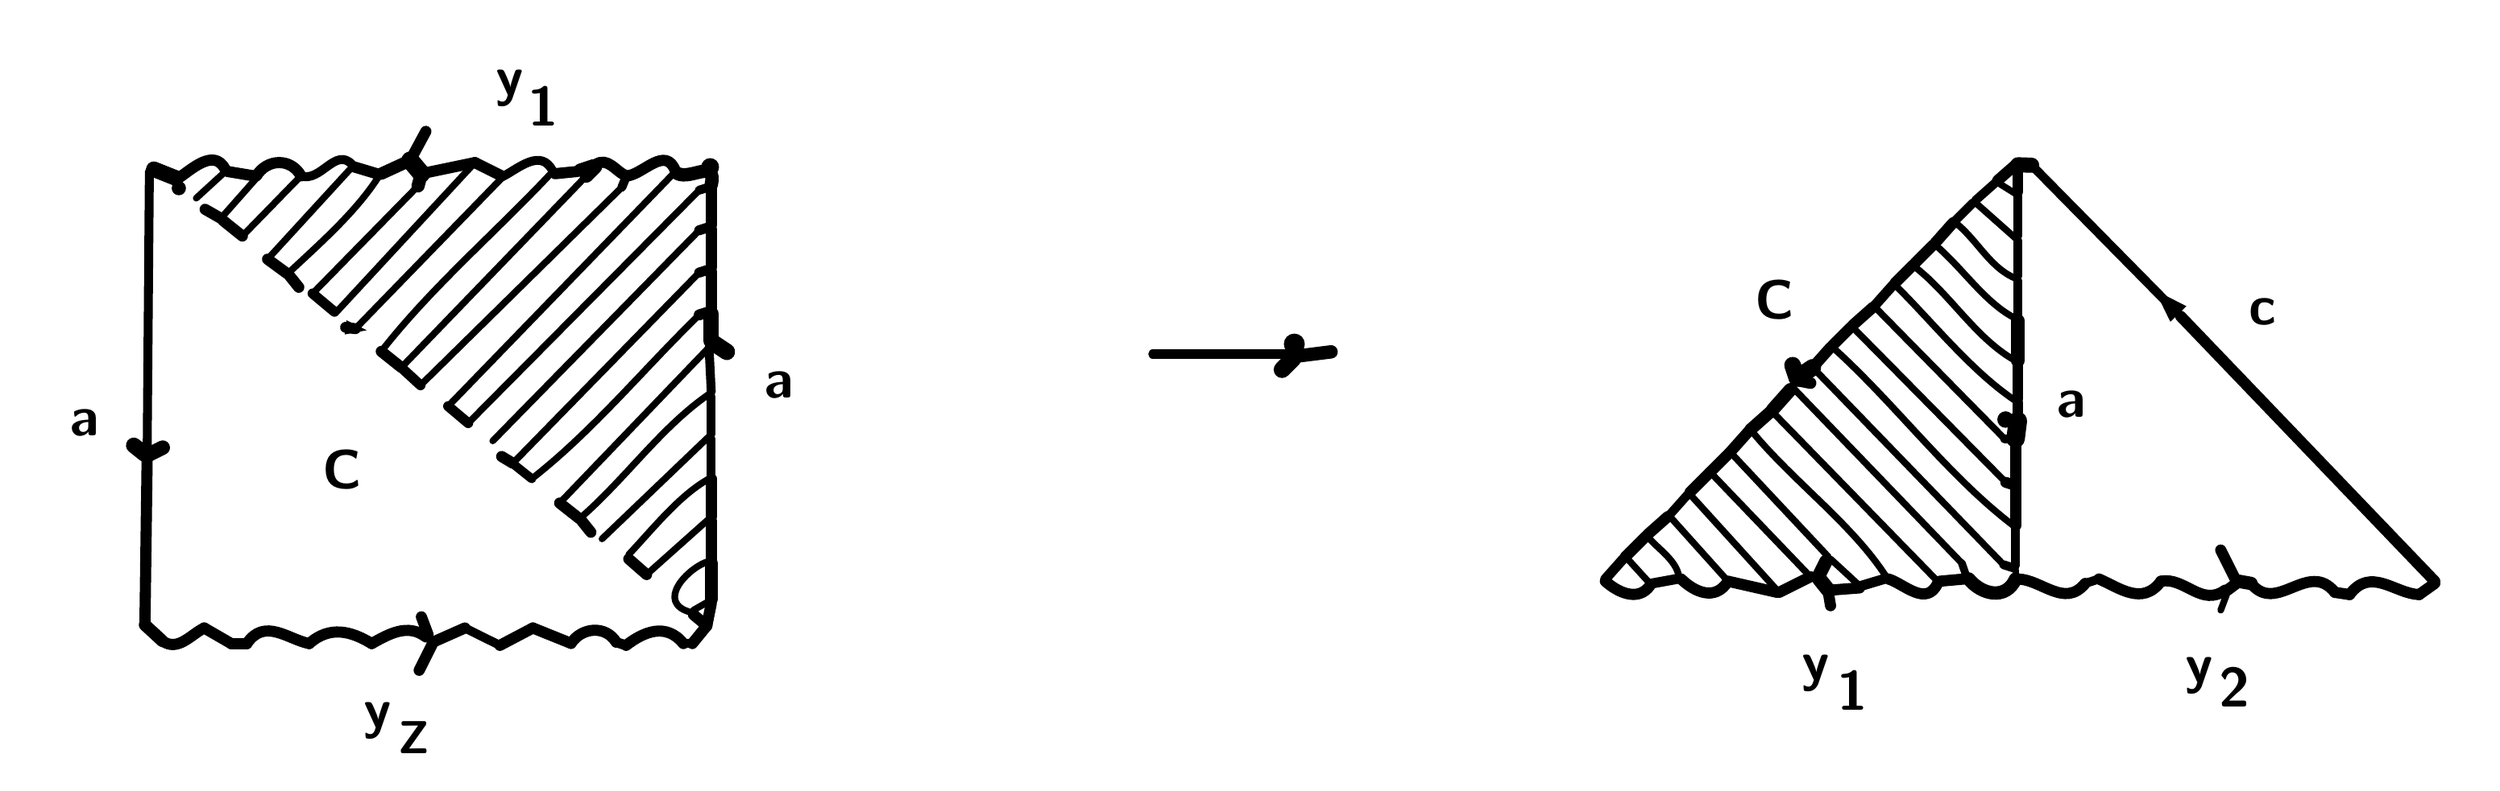
\begin{tikzpicture}[x=1pt, y=-1pt, line width=4.9pt, line cap=round, line join=round]

  %% ════ 填充区（prims2 的 fills）════

  %% ════ 直线段（prims2 的 strokes）════
  \draw[line width=4.9pt] (145.0,137.0) -- (149.4,137.6);
  \fill (144.6,140.2) -- (145.4,133.8) -- (154.5,138.3) -- cycle;
  \draw[line width=3.0pt] (149.4,137.6) -- (215.0,70.0);
  \draw[line width=5.0pt] (824.0,254.0) -- (811.0,255.0);
  \draw[line width=5.0pt] (104.0,69.0) -- (92.0,67.0);
  \draw[line width=7.0pt] (309.0,143.0) -- (309.0,131.0);
  \draw[line width=5.0pt] (120.0,114.0) -- (124.0,119.0);
  \draw[line width=5.0pt] (309.0,222.0) -- (309.0,205.0);
  \draw[line width=3.0pt] (894.0,77.0) -- (886.0,72.0);
  \draw[line width=6.0pt] (809.0,242.0) -- (806.0,248.0);
  \draw[line width=5.1pt] (993.0,252.0) -- (989.0,255.0);
  \draw[line width=4.5pt] (831.0,127.0) -- (839.0,118.0);
  % （略）线段 (968.0,131.0)-(973.0,129.0) 线宽5.7 —— 是箭头头那一坨，已由箭头头代替
  \draw[line width=5.0pt] (986.0,237.0) -- (993.0,251.0);
  \draw[line width=4.5pt] (718.0,241.0) -- (710.0,250.0);
  \draw[line width=5.0pt] (309.0,241.0) -- (309.0,224.0);
  \draw[line width=4.0pt] (308.0,74.0) -- (303.6,75.4);
  \draw[line width=3.0pt] (303.6,75.4) -- (201.0,179.0);
  \draw[line width=5.0pt] (161.0,147.8) -- (170.0,155.0);
  \draw[line width=4.0pt] (876.0,80.0) -- (885.0,72.0);
  \draw[line width=7.6pt] (797.0,159.0) -- (803.0,155.0);
  \draw[line width=5.0pt] (849.0,108.0) -- (857.0,100.0);
  \draw[line width=4.5pt] (200.0,180.0) -- (191.0,172.4);
  \draw[line width=3.0pt] (191.0,172.4) -- (292.0,68.0);
  \draw[line width=5.0pt] (119.0,113.0) -- (110.0,106.4);
  \draw[line width=3.0pt] (110.0,106.4) -- (147.0,66.0);
  \draw[line width=5.0pt] (858.0,99.0) -- (866.0,90.0);
  \draw[line width=3.0pt] (308.0,260.0) -- (301.0,264.0);
  \draw[line width=5.0pt] (251.0,224.0) -- (255.0,229.0);
  \draw[line width=3.0pt] (802.0,249.0) -- (757.0,202.0);
  \draw[line width=3.0pt] (802.0,249.0) -- (805.0,249.0);
  \draw[line width=5.0pt] (802.0,249.0) -- (788.0,256.0);
  \draw[line width=5.0pt] (215.0,69.0) -- (203.0,63.0);
  \draw[line width=5.0pt] (272.0,241.0) -- (280.0,248.0);
  \draw[line width=3.0pt] (280.0,248.0) -- (308.0,223.0);
  \draw[line width=4.0pt] (967.0,131.0) -- (901.2,64.2);
  \fill (970.6,127.5) -- (963.4,134.5) -- (956.5,120.3) -- cycle;
  \draw[line width=6.8pt] (901.2,64.2) -- (895.0,64.0);
  \draw[line width=5.3pt] (802.0,162.0) -- (797.0,161.0);
  \draw[line width=6.0pt] (785.0,174.0) -- (793.0,165.0);
  \draw[line width=5.0pt] (250.0,223.0) -- (241.0,215.9);
  \draw[line width=3.0pt] (241.0,215.9) -- (308.0,146.0);
  \draw[line width=4.0pt] (895.0,132.0) -- (895.0,116.0);
  \draw[line width=3.0pt] (811.0,241.0) -- (824.0,253.0);
  \draw[line width=4.5pt] (731.0,252.0) -- (742.0,250.0);
  \draw[line width=4.0pt] (894.0,227.0) -- (894.0,244.0);
  \draw[line width=5.0pt] (89.0,88.0) -- (82.0,84.0);
  \draw[line width=5.0pt] (766.0,193.0) -- (774.0,184.0);
  \draw[line width=5.0pt] (766.0,193.0) -- (757.0,202.0);
  \draw[line width=3.0pt] (766.0,193.0) -- (810.0,240.0);
  \draw[line width=3.0pt] (894.0,246.0) -- (894.0,249.0);
  \draw[line width=4.0pt] (309.0,168.0) -- (309.0,185.0);
  \draw[line width=4.0pt] (739.0,221.0) -- (747.0,212.0);
  \draw[line width=4.0pt] (931.4,250.0) -- (925.2,252.0);
  \draw[line width=5.0pt] (894.0,208.0) -- (894.0,188.0);
  \draw[line width=4.9pt] (894.0,208.0) -- (889.6,206.6);
  \draw[line width=3.0pt] (889.6,206.6) -- (821.0,137.0);
  \draw[line width=5.0pt] (894.0,208.0) -- (894.0,226.0);
  \draw[line width=6.0pt] (571.0,150.0) -- (587.0,148.0);
  \draw[line width=4.0pt] (309.0,187.0) -- (309.0,204.0);
  \draw[line width=5.0pt] (894.0,64.0) -- (886.0,71.0);
  \draw[line width=5.0pt] (811.0,146.0) -- (803.0,155.0);
  \draw[line width=5.0pt] (249.0,67.0) -- (239.0,68.0);
  \draw[line width=5.0pt] (185.0,278.0) -- (198.5,272.0);
  \draw[line width=4.0pt] (198.5,272.0) -- (214.2,279.8);
  \draw[line width=5.0pt] (214.2,279.8) -- (229.0,272.0);
  \draw[line width=5.0pt] (229.0,272.0) -- (246.1,278.9);
  \draw[line width=4.5pt] (266.4,278.4) -- (270.8,279.8);
  \draw[line width=4.0pt] (296.5,279.0) -- (300.5,279.0);
  \draw[line width=5.0pt] (300.5,279.0) -- (307.0,271.0);
  % （略）线段 (965.0,138.0)-(966.0,132.0) 线宽6.3 —— 是箭头头那一坨，已由箭头头代替
  \draw[line width=5.0pt] (820.0,137.0) -- (812.0,145.0);
  \draw[line width=5.0pt] (860.0,251.0) -- (871.0,250.0);
  \draw[line width=5.0pt] (181.0,49.0) -- (174.0,62.0);
  % （略）线段 (152.0,131.0)-(144.0,133.0) 线宽8.6 —— 是箭头头那一坨，已由箭头头代替
  \draw[line width=5.5pt] (174.0,62.0) -- (161.0,68.0);
  \draw[line width=8.0pt] (174.0,62.0) -- (179.0,68.0);
  \draw[line width=4.0pt] (569.0,149.0) -- (507.0,149.0);
  \draw[line width=7.0pt] (55.0,194.0) -- (50.0,190.0);
  \draw[line width=3.0pt] (105.0,70.0) -- (90.0,87.0);
  \draw[line width=7.4pt] (310.0,144.0) -- (316.0,148.0);
  \draw[line width=4.0pt] (895.0,78.0) -- (895.0,96.0);
  \draw[line width=5.0pt] (728.0,231.0) -- (719.0,240.0);
  \draw[line width=3.0pt] (78.0,79.0) -- (90.0,68.0);
  \draw[line width=4.5pt] (835.0,250.0) -- (825.0,253.0);
  \draw[line width=3.0pt] (894.0,97.0) -- (876.0,81.0);
  \draw[line width=4.5pt] (171.0,156.0) -- (178.6,163.0);
  \draw[line width=3.0pt] (178.6,163.0) -- (268.9,74.1);
  \draw[line width=4.0pt] (268.9,74.1) -- (271.0,69.0);
  \draw[line width=5.0pt] (90.0,89.0) -- (98.7,96.0);
  \draw[line width=3.0pt] (98.7,96.0) -- (125.0,69.0);
  \draw[line width=3.0pt] (260.0,232.0) -- (308.0,186.0);
  \draw[line width=5.0pt] (179.0,68.0) -- (203.0,63.0);
  \draw[line width=5.9pt] (179.0,68.0) -- (177.5,73.5);
  \draw[line width=3.0pt] (177.5,73.5) -- (130.2,121.8);
  \draw[line width=4.5pt] (130.2,121.8) -- (140.0,130.0);
  \draw[line width=4.0pt] (867.0,89.0) -- (875.0,81.0);
  \draw[line width=5.0pt] (895.0,176.0) -- (895.0,171.0);
  \draw[line width=6.6pt] (810.0,255.0) -- (806.0,250.0);
  \draw[line width=5.0pt] (968.0,132.0) -- (1082.0,251.0);
  \draw[line width=3.0pt] (141.0,130.0) -- (203.0,63.0);
  \draw[line width=5.0pt] (250.0,66.0) -- (256.0,64.0);
  \draw[line width=5.0pt] (309.0,261.0) -- (307.0,271.0);
  \draw[line width=3.0pt] (787.0,255.0) -- (748.0,212.0);
  \draw[line width=7.5pt] (796.0,160.0) -- (794.0,154.0);
  \draw[line width=8.3pt] (895.0,179.0) -- (894.0,187.0);
  \draw[line width=3.0pt] (831.0,128.0) -- (889.0,187.0);
  \draw[line width=4.0pt] (889.0,187.0) -- (893.0,187.0);
  \draw[line width=3.0pt] (989.0,256.0) -- (986.0,264.0);
  \draw[line width=5.0pt] (840.0,117.0) -- (848.0,109.0);
  \draw[line width=3.0pt] (739.0,222.0) -- (765.0,251.0);
  \draw[line width=4.0pt] (57.0,67.0) -- (56.0,193.0);
  \draw[line width=5.0pt] (215.0,195.0) -- (220.0,198.0);
  \draw[line width=5.0pt] (821.0,136.0) -- (830.0,128.0);
  \draw[line width=5.0pt] (757.0,202.0) -- (748.0,211.0);
  \draw[line width=4.0pt] (221.0,199.0) -- (228.5,205.0);
  \draw[line width=4.9pt] (303.6,131.4) -- (308.0,130.0);
  \draw[line width=3.0pt] (785.0,175.0) -- (859.0,251.0);
  \draw[line width=5.0pt] (100.7,279.0) -- (93.7,279.0);
  \draw[line width=5.0pt] (93.7,279.0) -- (81.6,272.0);
  \draw[line width=5.5pt] (62.8,277.8) -- (55.0,270.6);
  \draw[line width=5.0pt] (55.0,270.6) -- (56.0,195.0);
  \draw[line width=4.0pt] (309.0,166.0) -- (308.0,146.0);
  \draw[line width=3.0pt] (803.0,155.0) -- (888.6,243.6);
  \draw[line width=4.0pt] (888.6,243.6) -- (893.0,245.0);
  \draw[line width=5.0pt] (178.0,291.0) -- (184.0,279.0);
  \draw[line width=6.0pt] (895.0,152.0) -- (895.0,134.0);
  \draw[line width=4.0pt] (895.0,114.0) -- (895.0,98.0);
  \draw[line width=5.5pt] (775.0,183.0) -- (784.0,175.0);
  \draw[line width=5.0pt] (895.0,65.0) -- (895.0,76.0);
  \draw[line width=3.0pt] (730.0,252.0) -- (720.0,241.0);
  \draw[line width=6.1pt] (257.0,65.0) -- (253.0,69.0);
  \draw[line width=3.0pt] (211.0,188.0) -- (303.6,93.4);
  \draw[line width=4.5pt] (303.6,93.4) -- (308.0,92.0);
  \draw[line width=6.5pt] (63.0,191.0) -- (57.0,194.0);
  \draw[line width=7.0pt] (59.0,66.0) -- (69.0,70.0);
  \draw[line width=5.0pt] (179.0,267.0) -- (182.0,275.0);
  \draw[line width=6.0pt] (994.0,251.0) -- (999.6,252.0);
  \draw[line width=5.0pt] (1037.2,256.0) -- (1043.8,257.0);
  \draw[line width=5.0pt] (1075.0,257.0) -- (1082.0,252.0);
  \draw[line width=5.0pt] (307.0,271.0) -- (301.0,266.0);
  \draw[line width=5.0pt] (765.0,251.0) -- (787.0,256.0);
  \draw[line width=5.0pt] (309.0,93.0) -- (309.0,110.0);
  \draw[line width=4.5pt] (308.0,111.0) -- (303.6,112.4);
  \draw[line width=3.0pt] (303.6,112.4) -- (221.0,197.0);
  \draw[line width=5.0pt] (309.0,112.0) -- (309.0,129.0);
  \draw[line width=3.0pt] (171.0,154.0) -- (252.0,70.0);
  \draw[line width=5.0pt] (309.0,74.0) -- (309.0,91.0);
  \draw[line width=3.0pt] (795.0,165.0) -- (869.9,242.9);
  \draw[line width=3.5pt] (869.9,242.9) -- (872.0,249.0);
  \draw[line width=6.0pt] (309.0,259.0) -- (309.0,243.0);
  \draw[line width=5.0pt] (810.0,256.0) -- (811.0,262.0);
  \draw[line width=5.0pt] (895.0,169.0) -- (895.0,153.0);
  \draw[line width=7.5pt] (565.0,156.0) -- (570.0,151.0);
  \draw[line width=5.0pt] (159.0,68.0) -- (149.0,65.0);
  \draw[line width=5.0pt] (738.0,222.0) -- (729.0,230.0);

  %% ════ 曲线（prims2 的 curves —— 三段式，坐标同为 (y,x)）════
  \draw[line width=4.0pt] (216.0,69.0) .. controls (222.5,65.6) and (232.8,56.3) .. (238.0,67.0);
  \draw[line width=3.0pt] (272.0,239.0) .. controls (283.0,227.3) and (294.8,212.3) .. (308.0,205.0);
  \draw[line width=3.0pt] (237.0,68.0) .. controls (211.7,94.9) and (183.2,119.3) .. (161.0,147.8);
  \draw[line width=5.0pt] (257.0,64.0) .. controls (262.5,60.0) and (266.3,67.3) .. (271.0,69.0);
  \draw[line width=3.0pt] (812.0,146.0) .. controls (840.3,171.5) and (863.6,203.6) .. (893.0,226.0);
  \draw[line width=6.0pt] (873.0,250.0) .. controls (878.6,256.9) and (889.5,259.8) .. (894.0,250.0);
  \draw[line width=5.0pt] (988.0,255.0) .. controls (977.3,262.7) and (969.9,249.0) .. (959.2,251.0);
  \draw[line width=5.0pt] (959.2,251.0) .. controls (950.9,262.3) and (940.3,253.8) .. (931.4,250.0);
  \draw[line width=5.0pt] (925.2,252.0) .. controls (916.0,263.2) and (905.6,250.2) .. (895.0,250.0);
  \draw[line width=3.0pt] (894.0,170.0) .. controls (874.1,156.6) and (857.4,135.3) .. (840.0,118.0);
  \draw[line width=5.0pt] (246.1,278.9) .. controls (250.8,271.7) and (261.6,270.6) .. (266.4,278.4);
  \draw[line width=5.0pt] (270.8,279.8) .. controls (278.8,273.6) and (288.8,269.5) .. (296.5,279.0);
  \draw[line width=6.0pt] (309.0,73.0) .. controls (311.4,61.1) and (300.3,70.7) .. (294.0,68.0);
  \draw[line width=3.0pt] (120.0,112.0) .. controls (134.2,98.7) and (150.0,84.8) .. (160.0,69.0);
  \draw[line width=3.0pt] (251.0,222.0) .. controls (270.9,204.5) and (286.8,181.6) .. (308.0,167.0);
  \draw[line width=5.0pt] (125.0,69.0) .. controls (120.5,60.8) and (109.7,61.2) .. (105.0,69.0);
  \draw[line width=4.0pt] (125.0,69.0) .. controls (133.9,72.0) and (140.6,55.7) .. (148.0,64.0);
  \draw[line width=3.0pt] (228.5,205.0) .. controls (256.0,183.5) and (278.7,155.6) .. (303.6,131.4);
  \draw[line width=5.0pt] (181.0,276.0) .. controls (172.8,269.7) and (164.1,274.9) .. (156.7,279.0);
  \draw[line width=5.0pt] (156.7,279.0) .. controls (147.4,273.3) and (137.8,270.9) .. (128.7,279.0);
  \draw[line width=5.0pt] (128.7,279.0) .. controls (119.3,277.2) and (108.7,267.2) .. (100.7,279.0);
  \draw[line width=5.0pt] (81.6,272.0) .. controls (75.6,274.9) and (69.8,282.8) .. (62.8,277.8);
  \draw[line width=3.0pt] (858.0,100.0) .. controls (870.3,110.4) and (880.3,126.1) .. (894.0,133.0);
  \draw[line width=3.0pt] (308.0,242.0) .. controls (298.6,244.7) and (283.4,260.7) .. (300.0,265.0);
  \draw[line width=5.0pt] (70.0,70.0) .. controls (75.6,66.4) and (85.9,56.2) .. (91.0,66.0);
  \draw[line width=3.0pt] (836.0,249.0) .. controls (820.5,225.1) and (794.6,206.5) .. (776.0,184.0);
  \draw[line width=3.0pt] (894.0,152.0) .. controls (876.5,142.4) and (864.8,122.3) .. (849.0,110.0);
  \draw[line width=5.0pt] (999.6,252.0) .. controls (1011.1,266.2) and (1025.3,241.2) .. (1037.2,256.0);
  \draw[line width=5.0pt] (1043.8,257.0) .. controls (1053.3,244.3) and (1064.1,256.6) .. (1075.0,257.0);
  \draw[line width=5.0pt] (765.0,251.0) .. controls (759.3,260.2) and (749.9,255.8) .. (744.0,250.0);
  \draw[line width=5.0pt] (293.0,67.0) .. controls (288.6,54.8) and (278.2,68.7) .. (271.0,69.0);
  \draw[line width=5.0pt] (859.0,252.0) .. controls (853.9,262.7) and (843.9,252.1) .. (837.0,250.0);
  \draw[line width=5.0pt] (710.0,251.0) .. controls (715.3,255.8) and (724.6,260.5) .. (730.0,253.0);
  \draw[line width=3.0pt] (867.0,90.0) .. controls (876.8,97.7) and (882.5,110.3) .. (894.0,115.0);
  \draw[line width=3.0pt] (743.0,249.0) .. controls (741.9,241.6) and (733.9,236.8) .. (729.0,231.0);

  %% ════ 实心点 ════
  \fill (308.5,65.0) circle (4.0);
  \fill (70.2,74.5) circle (3.2);
  \fill (570.5,144.5) circle (4.7);
  \fill (889.5,178.4) circle (3.7);

  %% ════ 标签（probe 直接给的 \node 行）════
  %% ⚠ 全部补了 fill=white：文字在最上层，否则与曲线交叉干扰
     \node[anchor=center,inner sep=0pt,fill=white,font=\fontsize{29.2}{36.4}\selectfont] at (218.7,29.7) {\textsf{\textbf{\textit{y}}}};   % box(210,17,17,22)
     \node[anchor=center,inner sep=0pt,fill=white,font=\fontsize{23.0}{28.7}\selectfont] at (233.7,37.9) {\textsf{\textbf{1}}};   % box(227,30,8,15)
     \node[anchor=center,inner sep=0pt,fill=white,font=\fontsize{23.4}{29.3}\selectfont] at (786.1,124.7) {\textsf{\textbf{\textit{C}}}};   % box(778,116,15,17)
     \node[anchor=center,inner sep=0pt,fill=white,font=\fontsize{31.4}{39.3}\selectfont] at (1004.8,130.1) {\textsf{\textbf{\textit{c}}}};   % box(996,120,16,17)
     \node[anchor=center,inner sep=0pt,fill=white,font=\fontsize{31.0}{38.7}\selectfont] at (339.5,163.0) {\textsf{\textbf{\textit{a}}}};   % box(331,153,15,17)
     \node[anchor=center,inner sep=0pt,fill=white,font=\fontsize{32.9}{41.1}\selectfont] at (919.1,171.6) {\textsf{\textbf{\textit{a}}}};   % box(910,161,16,18)
     \node[anchor=center,inner sep=0pt,fill=white,font=\fontsize{32.0}{40.0}\selectfont] at (28.1,180.1) {\textsf{\textbf{\textit{a}}}};   % box(19,170,16,17)
     \node[anchor=center,inner sep=0pt,fill=white,font=\fontsize{24.2}{30.3}\selectfont] at (143.6,200.7) {\textsf{\textbf{\textit{C}}}};   % box(135,192,16,17)
     \node[anchor=center,inner sep=0pt,fill=white,font=\fontsize{29.8}{37.3}\selectfont] at (804.7,292.2) {\textsf{\textbf{\textit{y}}}};   % box(796,279,17,23)
     \node[anchor=center,inner sep=0pt,fill=white,font=\fontsize{29.8}{37.3}\selectfont] at (976.7,293.2) {\textsf{\textbf{\textit{y}}}};   % box(968,280,17,23)
     \node[anchor=center,inner sep=0pt,fill=white,font=\fontsize{23.6}{29.6}\selectfont] at (992.1,298.9) {\textsf{\textbf{2}}};   % box(986,290,11,17)
     \node[anchor=center,inner sep=0pt,fill=white,font=\fontsize{23.7}{29.7}\selectfont] at (820.8,300.4) {\textsf{\textbf{1}}};   % box(814,292,8,16)
     \node[anchor=center,inner sep=0pt,fill=white,font=\fontsize{29.2}{36.4}\selectfont] at (159.7,313.7) {\textsf{\textbf{\textit{y}}}};   % box(151,301,17,22)
     \node[anchor=center,inner sep=0pt,fill=white,font=\fontsize{20.3}{25.4}\selectfont] at (175.7,321.2) {\textsf{\textbf{\textit{Z}}}};   % box(169,312,11,17)

  % 钉死画布：否则超出的图元/控制点会把页面撑大，1:1 回比就失准
  \pgfresetboundingbox
  \path[use as bounding box] (0,0) rectangle (1101,335);
\end{tikzpicture}
\end{document}

% ⚠ 待核清单（probe 拿不准，人眼过一遍）：
%   · 未识别/跳过：⑤ 跳过/未识别的字形
